% This is samplepaper.tex, a sample chapter demonstrating the
% LLNCS macro package for Springer Computer Science proceedings;
% Version 2.20 of 2017/10/04
%
\newcommand{\tabincell}[2]{\begin{tabular}{@{}#1@{}}#2\end{tabular}}
\documentclass[runningheads]{llncs}
%
\usepackage{graphicx}
% Used for displaying a sample figure. If possible, figure files should
% be included in EPS format.
%
% If you use the hyperref package, please uncomment the following line
% to display URLs in blue roman font according to Springer's eBook style:
% \renewcommand\UrlFont{\color{blue}\rmfamily}

\begin{document}
%
\title{Auction System}

\author{Group 3: Peter Hösch \and Sena Tarpan \and Yun Ye}

\institute{}
%
\maketitle              % typeset the header of the contribution

\section{Introduction}
Our goal in this project is to design an auction system which enables a seller to sell a single product to a group of buyers. The buyers can place bids on the product. The product will be sold to the buyer who placed the highest bid at a predefined end date for the price of said last bid.

\section{Project requirements analysis}
\subsection{Features}
The seller defines a start and end date for the auction, describes the product as well as a starting bid. The buyers get informed about the the details of the product, the end date and the current highest bid every time said bid changes. Nodes can join or leave the auction at any time. The system should be able to recognize if a buyer goes offline or if a server crashes and take appropriate action. The server should be able handle high amounts of buyers by delegating work to supplemental servers if needed. 

\begin{table}
\caption{Methods and Parameters of Servers and Clients.}\label{tab1}
\begin{tabular}{|l|l|l|}
\hline
& {\bfseries Server} & {\bfseries Client}\\
\hline
{\bfseries Methods} & \tabincell{}{self\_identification()\\server\_logic()\\request\_join()\\broadcast()\\ validation\_token()\\inter\_server\_communication()\\reply\_to\_client()\\election()\\
update\_data()\\
} & \tabincell{}{self\_identification()\\client\_logic()\\request\_join()\\raise\_bid()}\\
\hline
{\bfseries Parameter} & \tabincell{}{{\bfseries float} highest\_bid\\{\bfseries list} bid\_history\\
{\bfseries dict} customer\_list\\{\bfseries dict} server\_list\\
{\bfseries tuple} proxy\_server\_address} & \tabincell{}{{\bfseries tuple} proxy\_server\_address\\
{\bfseries float} highest\_bid\\{\bfseries float} current\_bid\\{\bfseries string} own\_cookie\\
{\bfseries boolean} winner}\\
\hline
\end{tabular}
\end{table}

\begin{figure}
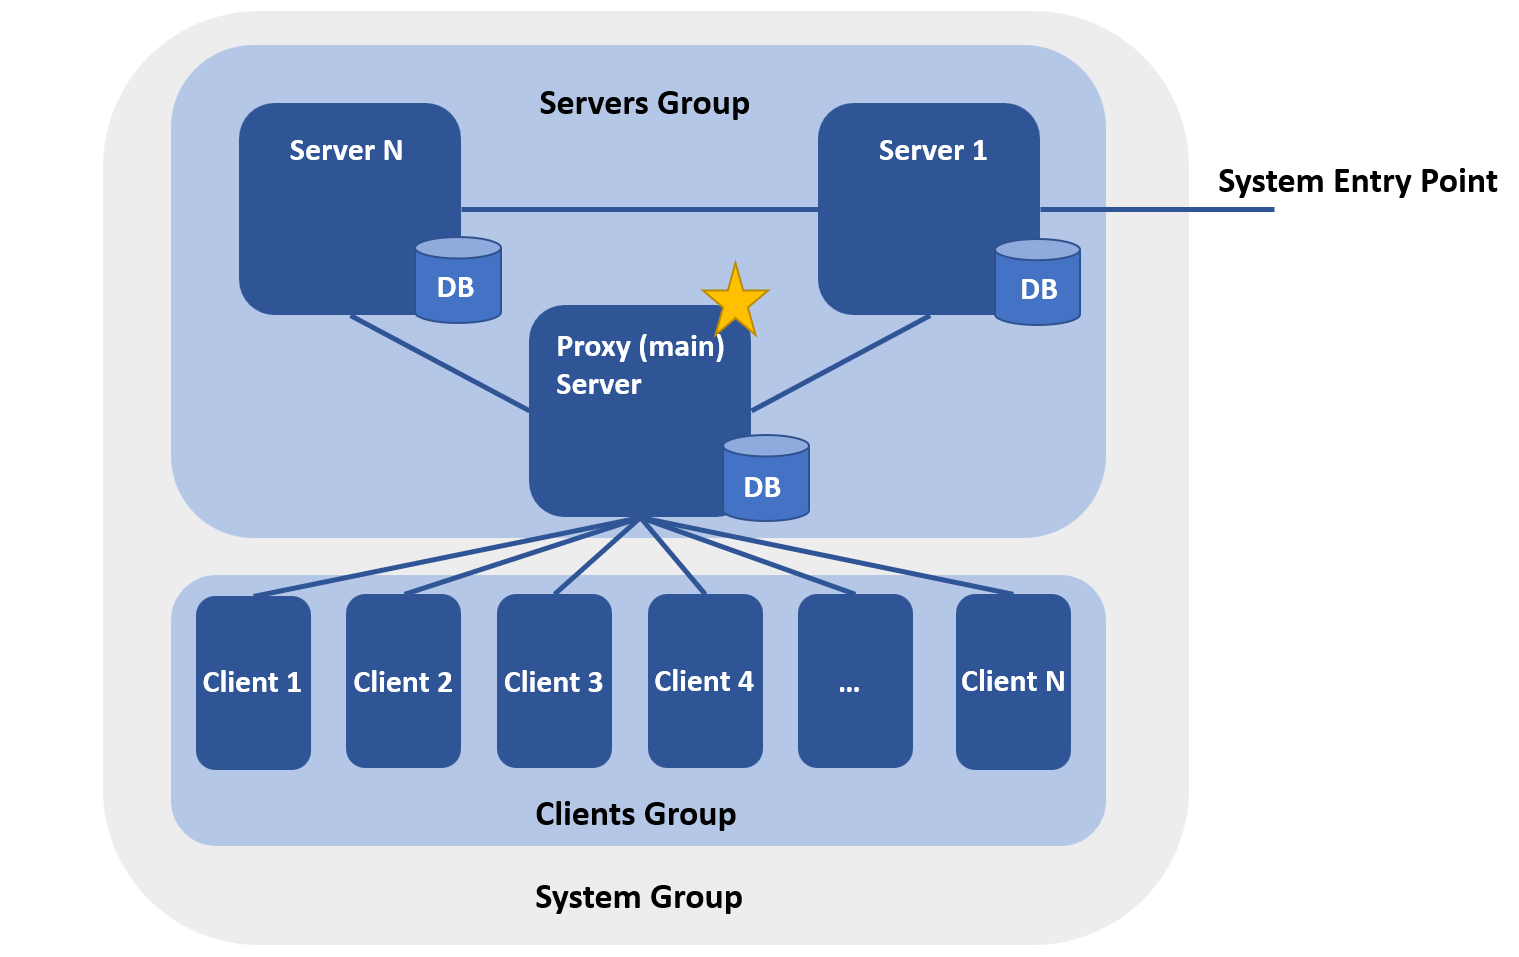
\includegraphics[width=\textwidth]{System Architecture.png}
\caption{Architecture diagram} \label{fig1}
\end{figure}

\subsection{Implementation}
The system will be implemented as a many servers-many clients design. The servers are the seller who functions as the main server as well as supplemental servers that provide fault tolerance and scalability. The clients on the other hand works like a think client machine that provide merely an interface with a very restrict logic and data functionality. Before the clients be token as one of the buyer, a validation cookie will be assigned to the client in case of some malicious party joining the Auction. Should the main server stop responding, the remaining servers will vote for a new main server from among their group. Otherwise, the supplemental servers exist to take bids, aggregate them and transfer that data to the main server. For this purpose, each server will be connected to a number of clients. The clients only communicate with this server, not directly with the main server or with each other. The servers will store a history of placed bids in case the connection to the leading bidder gets lost. In that case, the former second highest bid becomes the new highest bid and the clients get informed about this change. All servers maintain their own database and regularily synchronize with each other. To ensure that we become aware of lost connections or crashes, all participants in the auction are required to send a heartbeat signal in regular intervals to the server. If this signal doesn't arrives in a certain timeframe, the system will assume that the node that should havbe sent it is no longer available and proceed to initiate actions to replace them. Bids will be placed by using TCP connections from a client to a server to ensure that the bid will be reliably transported, while the servers will use UDP with ordered reliable multicast for the host discovery process, to inform all interested clients in a raised bid, and to regularily synchronize the current time which is important due to the time critical nature of an auction. If multiple bids with the same value get placed during a short timeframe the system should be able to determine which one was first and as such counts.

\begin{figure}
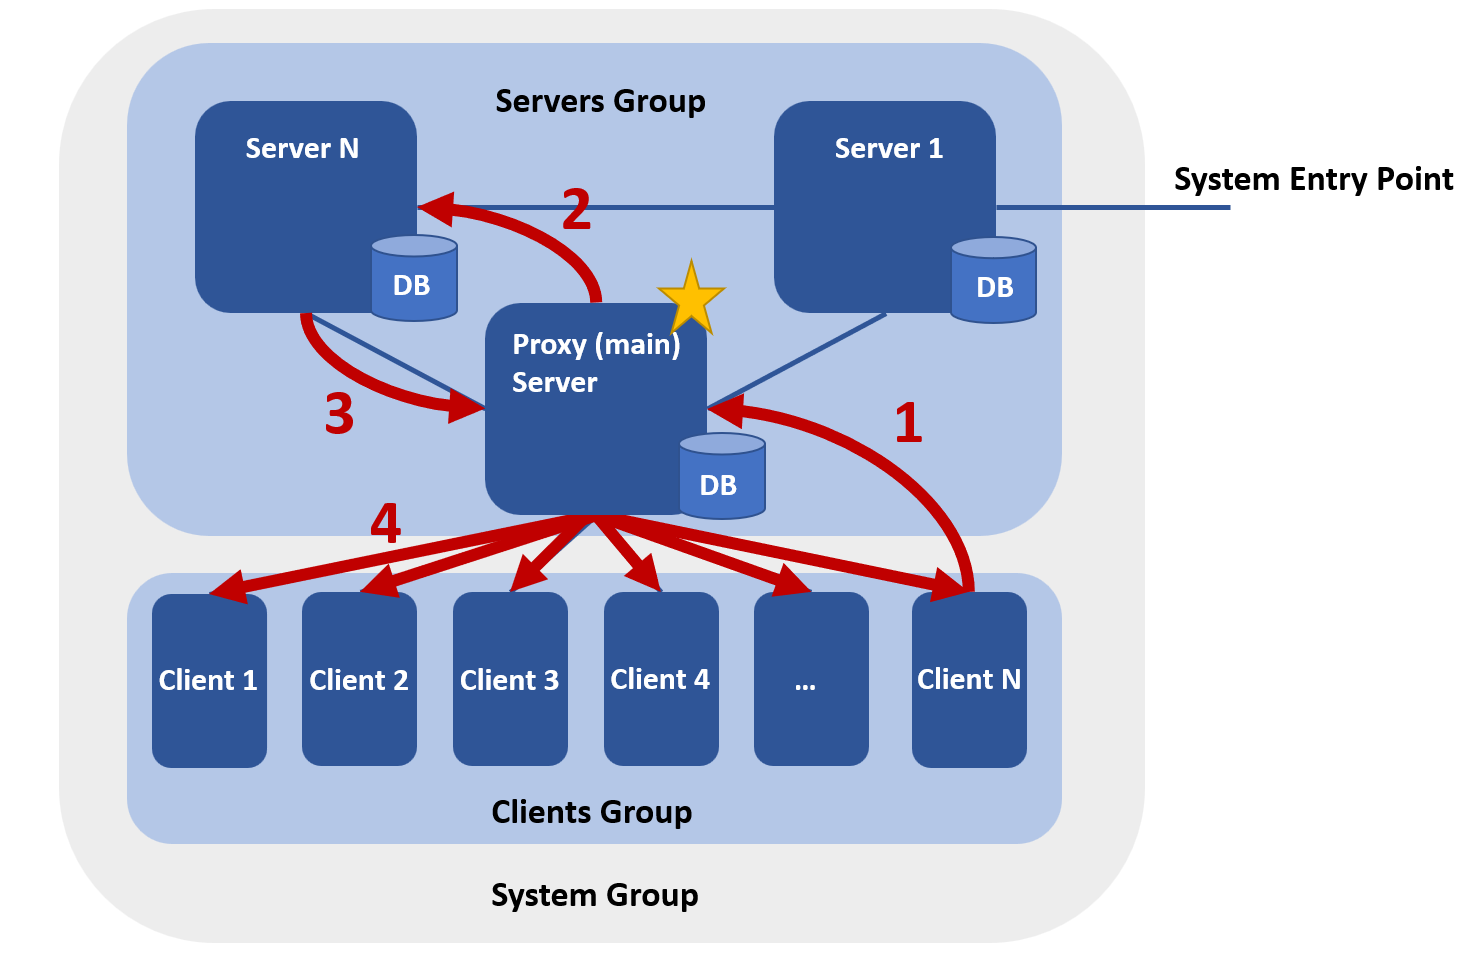
\includegraphics[width=\textwidth]{Raise Bid Example.png}
\caption{Raise Bid Example: 1.The Client send a json to Proxy Server through TCP. 2.The Proxy distribute the request to one of the server or handle the request itself. 3.The server send the result to Proxy. 4.The Proxy inform all the participants through UDP} \label{fig1}
\end{figure}

\end{document}
